\documentclass{beamer}

\mode<presentation> {
\usetheme{Madrid}
}

\beamertemplatenavigationsymbolsempty

\usepackage{pacman} % Allows you to be the best presentator ever :D

\usepackage{graphicx} % Allows including images
\usepackage{booktabs} % Allows the use of \toprule, \midrule and \bottomrule in tables
\usepackage[utf8]{inputenc}
\usepackage{float}
\usepackage{subcaption}
\usepackage{mathtools}
\usepackage{xcolor}
\usepackage{bm}

%-----------------------------------------------------------------------------
% Packages project-specified
%-----------------------------------------------------------------------------
\DeclareMathOperator{\Tr}{Tr}

%-----------------------------------------------------------------------------

%-----------------------------------------------------------------------------
%	TITLE PAGE
%-----------------------------------------------------------------------------

\title[ML - 2019/20 - Lorenzo Palloni]{Adversarially Constrained Autoencoder Interpolation using Wasserstein Autoencoder}
\subtitle{Machine Learning}
\author{Lorenzo Palloni}
\institute[]{
    University of Florence\\
    \medskip
    \textit{lorenzo.palloni@stud.unifi.it }
}
\date{\today}

\begin{document}

\begin{frame}
\titlepage % Print the title page as the first slide
\end{frame}

%-----------------------------------------------------------------------------
%	PRESENTATION SLIDES
%-----------------------------------------------------------------------------
%   TABLE OF CONTENTS
%-----------------------------------------------------------------------------
%\begin{frame}
%\tableofcontents
%\end{frame}
%-----------------------------------------------------------------------------
%-----------------------------------------------------------------------------
%-----------------------------------------------------------------------------
\begin{frame}
\frametitle{Introduction}
\begin{itemize}
  \item \textbf{Unsupervised Learning} context.
  \medskip
  \item We aim to obtain "high-quality" \textbf{interpolations}.
  \medskip
  \item An interpolation example:
\end{itemize}
\ \ \ \ \ \ $\overbrace{\ \ \ \ \ \ \ \ \ \ \ \ \ \ \ \ \ \ \ \ \ \ \ \ \ \ \ \ \ \ \ \ \ \ \ \ \ \ \ \ \ \ \ \ \ \ \ \ \ \ \ \ \ \ \ \ \ \ \ \ \ \ \ \ \ \ \ \ \ \ \ \ \ \ \ \ \ \ \ \ \ \ }^{\text{\textit{interpolated points}}}$
\vspace*{-\baselineskip}
\medskip
\begin{center}
  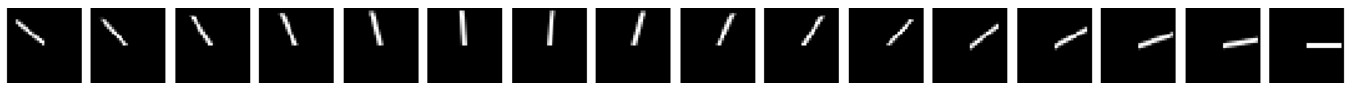
\includegraphics[width=1.0\textwidth,keepaspectratio]{./figures/perfect_interpolations}
\end{center}
\vspace*{-\baselineskip}
\begin{noindent}
  \rlap{\ \ $\nwarrow$} \hfill \llap{$\nearrow$\ \ }
\end{noindent}

\begin{noindent}
  \rlap{\textit{an endpoint}} \hfill \llap{\textit{another endpoint}}
\end{noindent}
\medskip
\begin{itemize}
  \item An "high-quality" interpolation point have two characteristics:
  \medskip
  \begin{itemize}
    \item is indistinguishable from real data;
    \medskip
    \item represents a semantically smooth morphing between the endpoints.
  \end{itemize}
\end{itemize}
\end{frame}
%-----------------------------------------------------------------------------
\begin{frame}
\frametitle{Motivation and Techniques}
\begin{itemize}
  \item Uncover underlying structure of dataset.
  \item Better representations $\rightarrow$ better results in other tasks.
\end{itemize}
\bigskip
\begin{itemize}
  \item Implemented\footnote{All the models are implemented using pytorch \cite{pytorch}} frameworks:
  \begin{itemize}
    \item Adversarially Constrained Autoencoder Interpolation (ACAI) \cite{acai};
    \medskip
    \item Wasserstein Autoencoder (WAE) \cite{wae};
  \end{itemize}
\end{itemize}
\end{frame}
%-----------------------------------------------------------------------------
\begin{frame}
\frametitle{ACAI}
\begin{itemize}
  \item Graphical representation of ACAI structure:
\end{itemize}
\begin{center}
  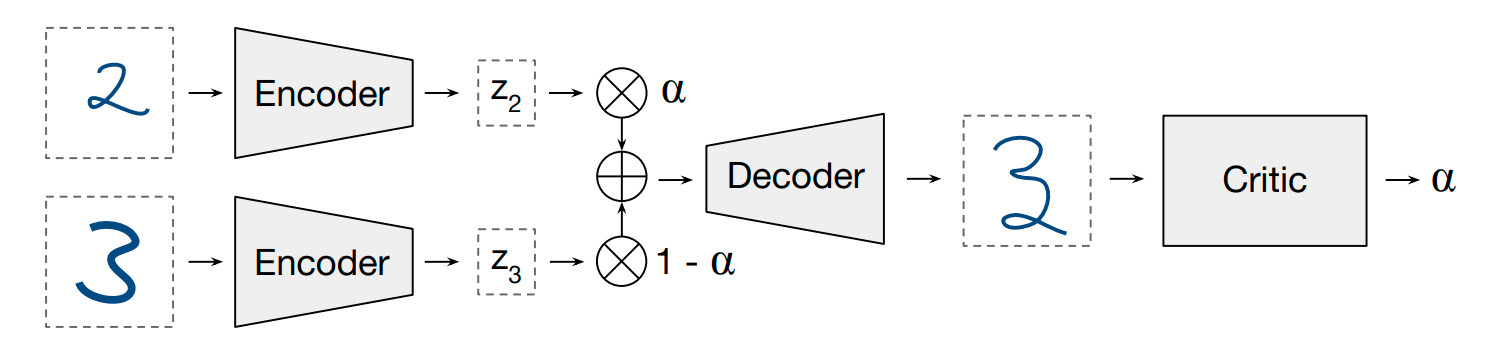
\includegraphics[width=\textwidth,keepaspectratio]{./figures/acai_structure}
\end{center}
\begin{itemize}
\onslide<2->{
  \item Loss functions:
}
\end{itemize}
\begin{align*}
\onslide<3->{
  \mathcal{L}_{d}&:=\left\|d_{\omega}\left(\hat{x}_{\alpha}\right)-\alpha\right\|^{2}+\left\|d_{\omega}\left(\gamma x+(1-\gamma) g_{\phi}\left(f_{\theta}(x)\right) \|^{2}\right.\right. \\
}
\onslide<4->{
  \mathcal{L}_{f, g}&:=\left\|x-g_{\phi}\left(f_{\theta}(x)\right)\right\|^{2}+\lambda\cdot\left\|d_{\omega}\left(\hat{x}_{\alpha}\right)\right\|^{2}
}
\end{align*}
\end{frame}
%-----------------------------------------------------------------------------
\begin{frame}
\frametitle{WAE}
\begin{itemize}
  \item Graphical representation of WAE structure:
\end{itemize}
\begin{center}
  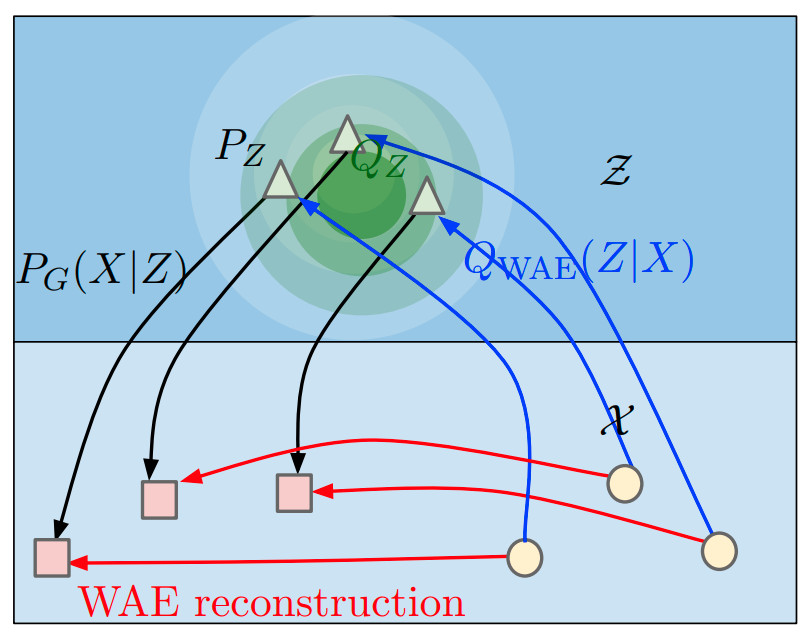
\includegraphics[width=0.50\textwidth,keepaspectratio]{./figures/wae_structure}
\end{center}
\begin{itemize}
  \item Loss function:
\end{itemize}
\begin{align*}
  D_{WAE}(P_X, P_G) := \inf_{Q(Z|X)\in\mathcal{Q}} \mathbb{E}_{P_X}\mathbb{E}_{Q(Z|X)}\left[c(X, G(Z))\right] + \lambda \cdot \mathcal{D}_Z(Q_Z, P_Z)
\end{align*}
\end{frame}
% %-----------------------------------------------------------------------------
% \begin{frame}
% \frametitle{Different penalties, different WAEs (1/3)}
% \begin{itemize}
%   \item Setting $$ \mathcal{D}_Z(Q_Z,P_Z) = D_{JS}(Q_Z, P_Z) $$
%   \item where $D_{JS}(\cdot,\cdot)$ is the Jensen-Shannon Divergence,
%   \medskip
%   \item[]$\rightarrow$ we obtain \textbf{WAE-GAN} (WAE using Generative Adversarial Network framework \cite{gan})
%   \medskip
%   \item A discriminator is introduced in order to estimate the $D_{JS}(P_Z,Q_Z)$.
%   \item Discriminator has to distinguish between $z\sim P_Z$ and $\tilde{z} \sim Q_Z$.
% %  \item where $D_{JS}(\cdot,\cdot)$ is the Jensen-Shannon Divergence:
% %  \begin{align}
% %    D_{JS}(Q_Z,P_Z) := \frac{1}{2} D_{KL}(Q_Z, \frac{Q_Z + P_Z}{2})
% %      + \frac{1}{2} D_{KL}(P_Z, \frac{Q_Z + P_Z}{2})
% %  \end{align}
% %  \item and $D_{KL}$ is the Kullback-Leibler Divergence:
% %  \begin{align}
% %    D_{KL}(Q_Z,P_Z) := \int Q_Z \log \left( \frac{Q_Z}{P_Z}\right )
% %  \end{align}
% \end{itemize}
% \end{frame}
%-----------------------------------------------------------------------------
\begin{frame}
\frametitle{Different penalties, different WAEs (1/2)}
\begin{itemize}
  \item Setting $$ \mathcal{D}_Z(Q_Z,P_Z) = MMD_k(Q_Z, P_Z) $$
  \vspace*{-\baselineskip}
  \item[]$\rightarrow$ \textbf{we obtain WAE-MMD}.
  \bigskip
  \item where $MMD_k(\cdot,\cdot)$ is the Maximum Mean Discrepancy \cite{mmd}:
  \begin{align*}
    MMD_\mathit{k}(Q_Z,P_Z) := \Big\| \int_{\mathcal{Z}} \mathit{k}(z, \cdot)dQ_Z(z) -
      \int_{\mathcal{Z}} \mathit{k}(z, \cdot)dP_Z(z)\Big\|_{\mathcal{H}_k}
  \end{align*}
  \item where $k$ is a positive-definite kernel $k$: $\mathcal{Z} \times \mathcal{Z} \rightarrow \mathcal{R} $.
\onslide<2->{
  \item Kernel used in the WAE paper:
  \begin{itemize}
}\onslide<3->{
    \item Radial Basis Function: $k(x, y) = \exp(-\gamma\left\| x - y \right\|^2)$
}\onslide<4->{
    \medskip
    \item Inverse Multiquadratic: $k(x, y) = \frac{C}{C + \left\| x - y \right\|^2},\ C \in \mathcal{R}$
  \end{itemize}
}
%  \item Unbiased empirical estimation of $MMD_k(Q_Z,P_Z)$ is given by:
%  {\footnotesize
%      $$
%      MMD_{\mathit{k}}(z, \tilde{z}) =
%        \frac{1}{n(n-1)} \sum_{i,j: i\neq j} \mathit{k}(z_i, z_j) +
%        \frac{1}{n(n-1)} \sum_{i,j: i\neq j} \mathit{k}(\tilde{z}_i, \tilde{z}_j) -
%        \frac{2}{n^2} \sum_{i,j: i\neq j} \mathit{k}(z_i, \tilde{z}_j)
%      $$
%  }
\end{itemize}
\end{frame}
%-----------------------------------------------------------------------------
\begin{frame}
\frametitle{Different penalties, different WAEs (2/2)}
\begin{itemize}
  \item Setting $$ \mathcal{D}_Z(Q_Z,P_Z) = \underbrace{\left\| \mu_{P_Z} - \mu_{Q_Z} \right\|^2 +
    \Tr \left( \Sigma_{P_Z} + \Sigma_{Q_Z} -
    2(\Sigma_{P_Z}\Sigma_{Q_Z})^{\frac{1}{2}} \right)}_{\text{2-Wasserstein distance between two multivariate normal distributions \cite{frechet}}} $$
  \item and assuming the prior $P_Z$ normal distributed,
  \item[] $\rightarrow$ \textbf{we obtain WWAE} (Wasserstein-Wasserstein Autoencoder) \cite{wwae}.
  \bigskip
\end{itemize}
\end{frame}
%-----------------------------------------------------------------------------
\begin{frame}
\frametitle{Roadmap of hands-on approach}
\begin{itemize}
  \item We aim to achieve "high-quality" interpolations on two datasets:
  \begin{itemize}
    \item MNIST (images)
    \item NESMDB \cite{nes} (music)
  \end{itemize}
\end{itemize}
\begin{enumerate}
\onslide<2->{
  \item ACAI + WAE applied on MNIST $\rightarrow$ poor results:
}
\onslide<3->{
  \begin{center}
    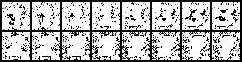
\includegraphics[width=0.4\textwidth,keepaspectratio]{./figures/acwae-epoch-28}
  \end{center}
}
\onslide<4->{
  \item ACAI + WAE applied on NESMDB $\rightarrow$ poor results too.
}
\onslide<5->{
  \item ACAI + WWAE applied on MNIST $\rightarrow$ good results (next slide).
}
\onslide<6->{
  \item ACAI + WWAE applied on NESMDB $\rightarrow$ requires too time to collect results.
}
\end{enumerate}
\end{frame}
%-----------------------------------------------------------------------------
\begin{frame}
\frametitle{Results on MNIST}
\begin{itemize}
  \item Example interpolations on MNIST made with ACAI + WWAE:
  \medskip
  \begin{center}
  \onslide<1->{
    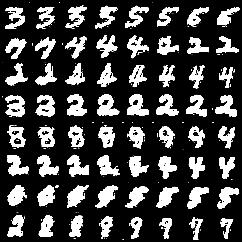
\includegraphics[width=0.4\textwidth]{./figures/01-mnist-interpolations}
  }
  \onslide<2->{
    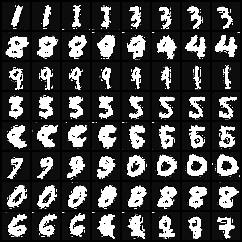
\includegraphics[width=0.4\textwidth]{./figures/02-mnist-interpolations}
  }
  \end{center}
  \item Each row is made by reconstructing (a sample) of the linear convex combination of the latent representation between the first and the last element of the row.
\end{itemize}
\end{frame}
%-----------------------------------------------------------------------------
\begin{frame}
\frametitle{Final discussions}
\begin{itemize}
  \item We achieve pretty good quality interpolations on image data using ACAI + WWAE.
  \medskip
  \item All models discussed so far require:
  \begin{itemize}
    \item high computational resources for training;
    \item have the lack of an objective way to assess the performance.
  \end{itemize}
  \medskip
  \item Raw audio in waveform probably needs:
  \begin{itemize}
    \item another type of representation (e.g. MIDI) \cite{music1} \cite{music2};
    \item another autoencoder structure (e.g. Wavenet Autoencoder \cite{wavenetae})
  \end{itemize}
%  \item An interesting application on raw audio could be Wavenet Autoencoder \cite{wavenetae} along side with ACAI framework.
\end{itemize}
\end{frame}
%-----------------------------------------------------------------------------
%-----------------------------------------------------------------------------
%-----------------------------------------------------------------------------
%-----------------------------------------------------------------------------
%-----------------------------------------------------------------------------
\begingroup
\footnotesize
\begin{frame}[allowframebreaks]
\frametitle{References}
\begin{thebibliography}{99}

\bibitem{acai}{Berthelot, David, et al. "Understanding and improving interpolation in autoencoders via an adversarial regularizer." arXiv preprint arXiv:1807.07543 (2018).}
\bibitem{wae}{Tolstikhin, Ilya, et al. "Wasserstein auto-encoders." arXiv preprint arXiv:1711.01558 (2017).}
\bibitem{wwae}{Zhang, Shunkang, et al. "Wasserstein-Wasserstein auto-encoders." arXiv preprint arXiv:1902.09323 (2019).}
\bibitem{pytorch}{Paszke, Adam, et al. "Automatic differentiation in pytorch." (2017).}
\bibitem{gan}{Goodfellow, Ian, et al. "Generative adversarial nets." Advances in neural information processing systems. 2014.}
\bibitem{frechet}{Dowson, D. C., and B. V. Landau. "The Fréchet distance between multivariate normal distributions." Journal of multivariate analysis 12.3 (1982): 450-455.}
\bibitem{music1}{Borghuis, Tijn, et al. "Off the Beaten Track: Using Deep Learning to Interpolate Between Music Genres." arXiv preprint arXiv:1804.09808 (2018).}
\bibitem{music2}{Borghuis, Tijn, et al. "Full-Band Music Genres Interpolations with Wasserstein Autoencoders." Ital-ia (2019).}
\bibitem{wavenetae}{Engel, Jesse, et al. "Neural audio synthesis of musical notes with wavenet autoencoders." Proceedings of the 34th International Conference on Machine Learning-Volume 70. JMLR. org, 2017.}
\bibitem{mmd}{Gretton, Arthur, et al. "A kernel two-sample test." Journal of Machine Learning Research 13.Mar (2012): 723-773.}
\bibitem{dcgan}{Radford, Alec, Luke Metz, and Soumith Chintala. "Unsupervised representation learning with deep convolutional generative adversarial networks." arXiv preprint arXiv:1511.06434 (2015).}
\bibitem{nes}{Donahue, Chris, Huanru Henry Mao, and Julian McAuley. "The NES music database: A multi-instrumental dataset with expressive performance attributes." arXiv preprint arXiv:1806.04278 (2018).}

\end{thebibliography}

\end{frame}
\endgroup
%-----------------------------------------------------------------------------
\begin{frame}
\frametitle{Appendix - Wasserstein distance}
\begin{itemize}
  \item Kantorovich's formulation of the \textit{optimal transport} problem:
  \begin{align*}
    W_c(P_X,P_G) := \inf_{\Gamma \in \mathcal{P} (X\sim P_X,Y_\sim P_G)}
    \mathbb{E}_{(X, Y)\sim \Gamma}\left[ c(X, Y) \right]
  \end{align*}
  \item with some weak constrains it could be written as the following:
  \begin{align*}
    W_1(P_X,P_G) = \sup_{f \in \mathcal{F}_{L_1}}
    \mathbb{E}_{X \sim P_X} \left[ f(X) \right] - \mathbb{E}_{Y \sim P_G} \left[ f(Y) \right]
  \end{align*}
  \item Moreover defining $P_G$ in two steps:
    \begin{enumerate}
      \item $Z \sim P_Z$
      \item $G: \mathcal{Z} \rightarrow \mathcal{R}^d$
    \end{enumerate}
  \item we have:
  \begin{align*}
    \inf_{\Gamma \in \mathcal{P} (X\sim P_X,Y_\sim P_G)}
    \mathbb{E}_{(X, Y)\sim \Gamma}\left[ c(X, Y) \right] =
    \inf_{Q:Q_Z=P_Z} \mathbb{E}_{Q(X|Z)} \left[ c(X, G(Z)) \right]
  \end{align*}
\end{itemize}
\end{frame}
%-----------------------------------------------------------------------------

\end{document}
